It has been recently recognized that existing protection mechanisms commonly implemented in Internet and distributed systems such as TCP checksums and redundant coding in storage systems are not sufficient to handle silent {\it gray failures}, which often lead to wide spread system slowdown, application malfunction, and corrupted data. As a result, advanced distributed systems started to add extra end-to-end data integrity checks to catch these failures early on in order to reduce application failures and blind retries~\cite{swip:pearc:2019}. 

However, identifying the root causes of these gray failures remains a largely unsolved problem due to the three grand challenges we scoped in Section~\ref{sec:introduction}: 
incomplete network state information, intermittent probabilistic nature of gray failures, and complexity in diagnosing complex networks in a scalable fashion.  

A network system can be modeled as a graph with a set of nodes connected by links via interfaces. The nodes in the network consist of end hosts (that generate and receive data) and networking devices (routers or switches). Due to scalability or privacy constraints, deploying monitoring capabilities at every point of the targeted large-scale network is not possible. Therefore, the problem can be concisely modeled as a bipartite mapping graph between the path level flows and its network components as shown in Fig.~\ref{fig:bipartite}. What makes the problem extremely difficult is that the mapping relationships in the bipartite graph are unknown. We further observe that one component failure (e.g., $L_j$) will cause multiple paths erroneous while one flow error (e.g., $F_i$) may be caused by multiple component failures. And because the component gray failure probability is normally low ($10^{-3} - 10^{-6}$), it would require large number of file transfers to catch a few number of corrupted files. Our ultimate goal is to localize the possible root causes in node or link errors by inference from the observed flow level abnormalities only at the end hosts, which can be translated to learning the mappings in such a graph.

\begin{wrapfigure}{ht}{0.26\textwidth}
\vspace{-10pt}
  \begin{center}
    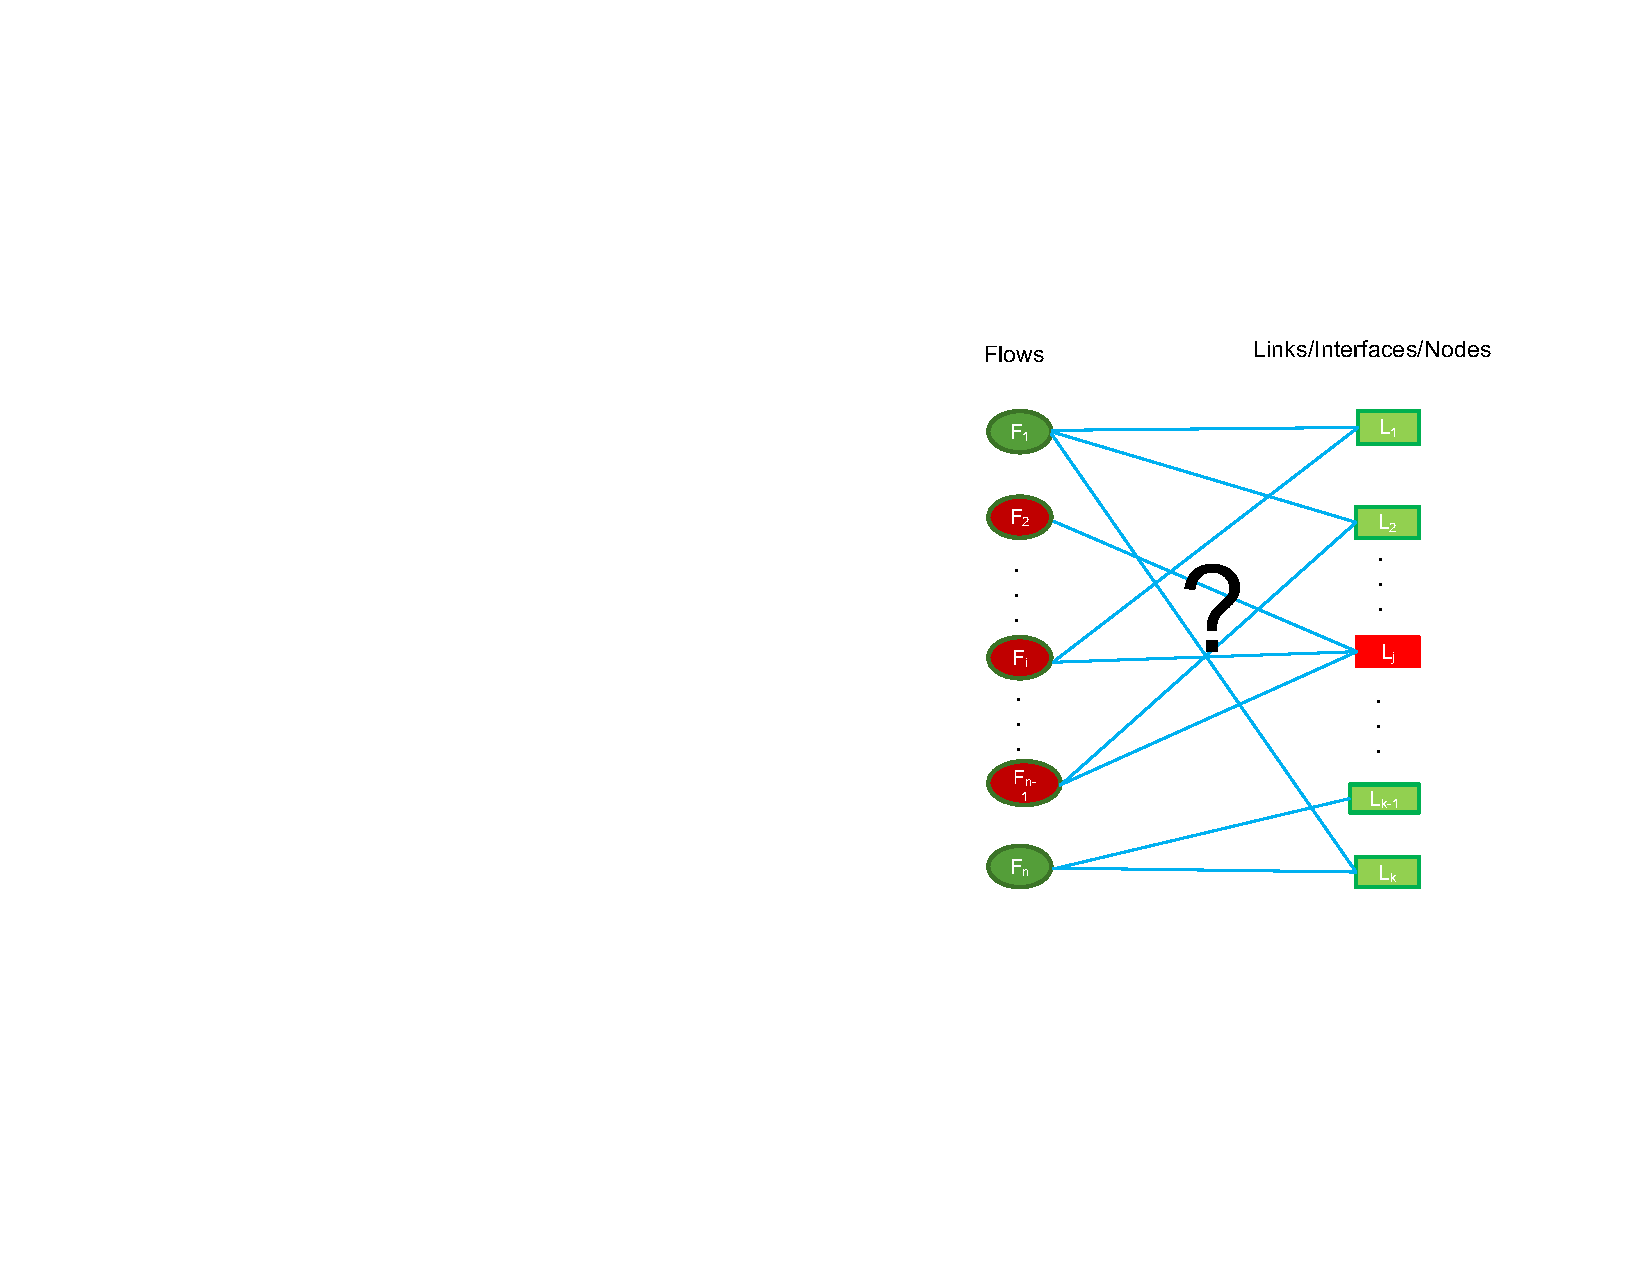
\includegraphics[width=0.26\textwidth]{./figure/RCABipartite}
  \end{center}
  \vspace{-5pt}
\caption{RCA Bipartite Graph}
\vspace{-5pt}
\label{fig:bipartite}
\end{wrapfigure}

The majority of recent work assume flow information between any pair of nodes in the network is available because they focus on data center networks that they have full ownership and modern routers allow originating and receiving probing data. This is very important because, as shown in~\cite{netbouncer:nsdi18}, there exists a minimal set of source-destination pairs to guarantee successful pinpointing of link errors in the network. Some of the work further assume they even know the routes of every flow, i.e., the mapping represented in Fig.~\ref{fig:bipartite}. However, both assumptions do not hold for our targeted multi-domain network environment due to obvious administrative constraints and the fact that, in the Internet scale network, traffic routing and forwarding are largely dynamically decided by the control plane software like OSPF and BGP subject to frequent topology and policy changes. 

We therefore made more restrictive but more realistic assumptions in this study in that (1) only the data file transfer information including integrity error states can be obtained at the end hosts from application layer; (2) only the physical nodes (domains) and their interfaces are known to us, but the network topology and traffic routing are unknown. 

In a large network, collecting the passive monitoring data from all node pairs may not scale well. Therefore injecting probe packets between the designated node pairs periodically is adapted by several existing RCA systems. In practice, due to the probabilistic nature of the grey failures, controlled fault injection is an efficient way to generate training data within a reasonable time frame.

Directly accessing the production system to instrument the analysis with either active probing or fault injection is not realistic in most cases, especially in a multi-domain system where no one owns the entire infrastructure like in the data center networks. We believe emulation with realistic scales is a viable choice, given advanced Cloud testbeds are available.








